\documentclass[12pt,letterpaper]{article}

\usepackage[utf8]{inputenc}
\usepackage[spanish]{babel}
\usepackage{graphicx}
\usepackage[hidelinks]{hyperref}
\usepackage{hyperref}
\usepackage[left=2cm,right=2cm,top=2.5cm,bottom=2cm]{geometry}
\usepackage{graphicx}
\usepackage{float}
\usepackage{amsmath}
\usepackage{stackrel} 
\usepackage{multicol}
\usepackage{multirow}
\usepackage{fancyhdr}
\usepackage[usenames,dvipsnames,svgnames,table]{xcolor}
\usepackage[document]{ragged2e}
\usepackage{enumerate}

\usepackage{helvet}

\renewcommand{\labelitemi}{$-$}
\renewcommand{\labelitemii}{$\cdot$}
\newcommand\tab[1][1cm]{\hspace*{#1}}

\renewcommand{\familydefault}{\sfdefault}

\definecolor{azul}{RGB}{0,0,255}

\pagestyle{fancy}
\lhead{\begin{picture}(0,0) \put(0,0){
\includegraphics[width=10mm]{./img/logo}} \end{picture}}
\chead{\hspace{1cm}\vspace{0.2cm}Laboratorio 02 - Importación, Data Flow, Traslado de archivos}
\rhead{}

\begin{document}
\begin{titlepage}
    \begin{center}
        \begin{figure}[htb]
            \begin{center}
                
\includegraphics[width=3.5cm]{./img/logo}
            \end{center}
        \end{figure}
        \vspace*{0.15in}
        \begin{Large}
            \textbf{UNIVERSIDAD PRIVADA DE TACNA}\\
        \end{Large}
        \vspace*{0.15in}
        \begin{Large}
            \textbf{FACULTAD DE INGENIERÍA} \\
        \end{Large}
        \vspace*{0.1in}
        \begin{Large}
            \textbf{Escuela Profesional de Ingeniería de Sistemas} \\
        \end{Large}
        \vspace*{0.3in}
        \begin{Large}
            \textbf{Laboratorio 02}\\
            \textbf{``Importación, Data Flow, Traslado de archivos"}\\
        \end{Large}
        \vspace*{0.2in}
        \begin{Large}
            \textbf{CURSO:} \\
        \end{Large}
        \vspace*{0.1in}
        \begin{large}
            Inteligencia de Negocios\\
        \end{large}
        \vspace*{0.2in}
        \begin{Large}
            \textbf{DOCENTE:} \\
        \end{Large}
        \vspace*{0.1in}
        \begin{large}
            Mag. Patrick Jose Cuadros Quiroga\\
        \end{large}
        \vspace*{0.3in}
        \begin{large}
            \textbf{ALUMNO:} \\
            \begin{flushleft}
                Lipa Calabilla, Abraham  		\hfill	(2019064039) \\
            \end{flushleft}
        \end{large}
        \vspace*{1.3in}
        \begin{large}
            Tacna - Perú\\
        \end{large}
        \vspace*{0.1in}
        \begin{large}
            2022\\
        \end{large}
    \end{center}
\end{titlepage}
\include{Secciones/articulo}
\newpage
\tableofcontents
\justify
\newpage
\begin{LARGE}
    \begin{center}
        \textbf{IMPORTACIÓN, DATA FLOW, TRASLADO DE ARCHIVOS} \\
    \end{center}
\end{LARGE}
\section{OBJETIVOS}
\begin{itemize}
    \item Importar datos usando el Wizard
    \item Desarrollar mis primeros paquetes DTSX
\end{itemize}

\section{REQUERIMIENTOS}
\begin{itemize}
    \item Conocimientos\\
          Para el desarrollo de esta práctica se requerirá de los siguientes conocimientos básicos:
          \begin{itemize}
              \item Conocimientos básicos de administración de base de datos Microsoft SQL Server.
              \item Conocimientos básicos de Visual Studio 2019.
          \end{itemize}
    \item Software\\
          Así mismo se necesitan los siguientes aplicativos:
          \begin{itemize}
              \item SQL Server Integration Services
              \item Base de datos Adventure Work (OLTP Y Datawarehouse) y AdventureWorksLT2012
              \item Microsoft SQL Server 2016 o superior
              \item Visual Studio 2019
          \end{itemize}
\end{itemize}

\section{CONSIDERACIONES INICIALES}
\begin{itemize}
    \item Tener todos los componentes considerados en los requerimientos de modo que se puedan crear Integration Services Projects
\end{itemize}

\newpage
\section{DESARROLLO}
\subsection{Tarea 1: Importación de datos usando el Wizard - SQL Management}
Crear una base de datos - BDTEST
Importar Datos desde AdventureWorks

\begin{center}
    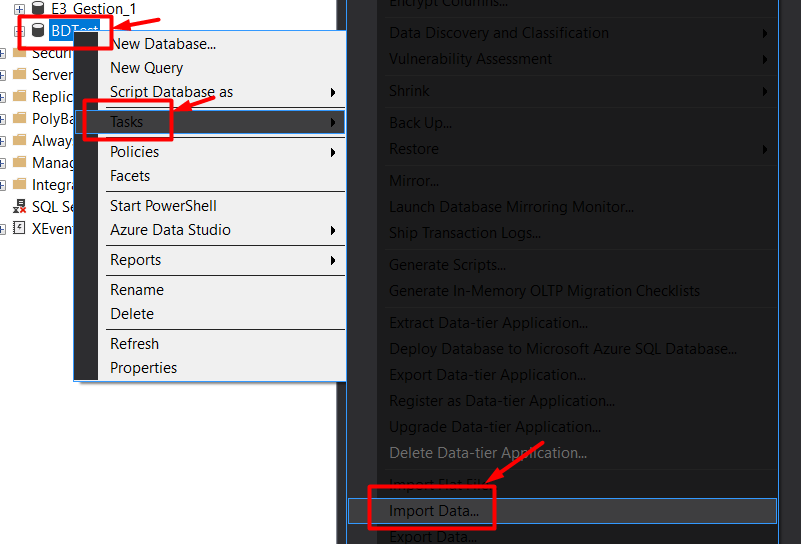
\includegraphics[width=10cm]{./img/img1.png}
\end{center}

Next y escribir el Servidor y seleccionar la base de datos

\begin{center}
    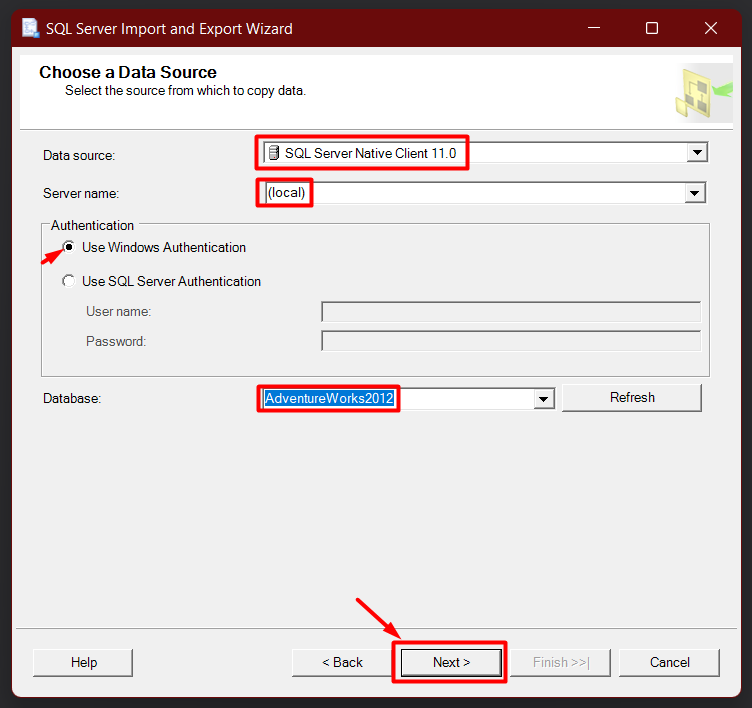
\includegraphics[width=10cm]{./img/img2.png}
\end{center}

\begin{center}
    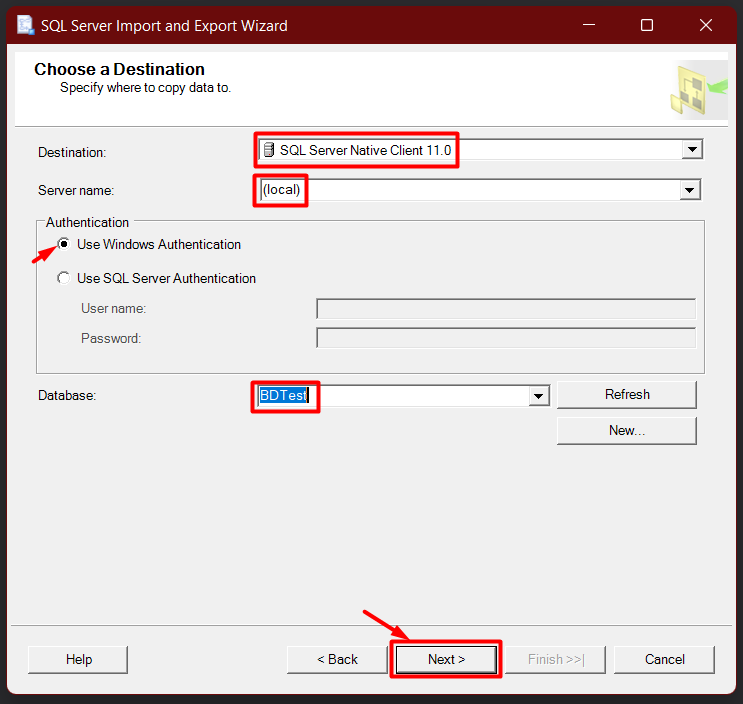
\includegraphics[width=10cm]{./img/img3.png}
\end{center}

\textbf{Data Source:} La base de donde vamos a importar

\textbf{Destination:} La Base donde vamos a cargar la data\\

Seleccionamos la primera opción

\begin{center}
    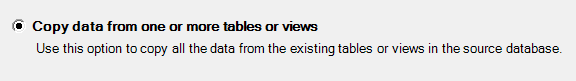
\includegraphics[width=13cm]{./img/img4.png}
\end{center}

Seleccionamos las dos tablas indicadas

\begin{center}
    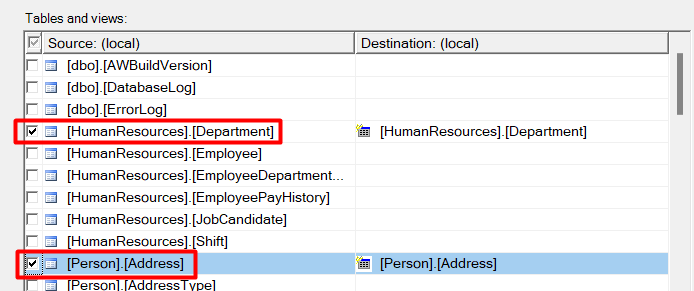
\includegraphics[width=10cm]{./img/img5.png}
\end{center}

Seleccionamos la opción para guardar el paquete SSIS como archivo

\begin{center}
    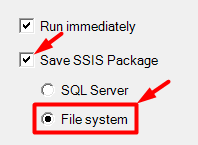
\includegraphics[width=5cm]{./img/img6.png}
\end{center}

Ingresamos el nombre y la ubicación

\begin{center}
    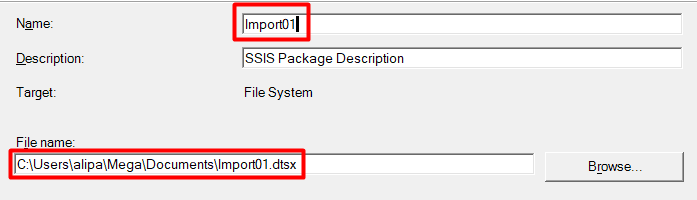
\includegraphics[width=10cm]{./img/img7.png}
\end{center}

Hacemos clic en Finish

\begin{center}
    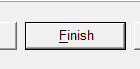
\includegraphics[width=5cm]{./img/img8.png}
\end{center}

Al finalizar, tenemos el resumen de la ejecución.

\begin{enumerate}[a. ]
    \item Hemos Generado nuestro 1 paquete de forma automática.
    \item Podemos actualizar la base de datos
    \item BdTest y encontraremos las tablas ya importadas.
\end{enumerate}

Con este procedimiento puede usted importar 5 tablas de BD Adventure Works a nuestra base de datos.

\subsection{Tarea 2: Creamos nuestro primer paquete DTSX}

Creamos un nuevo Integration Services Project

\begin{center}
    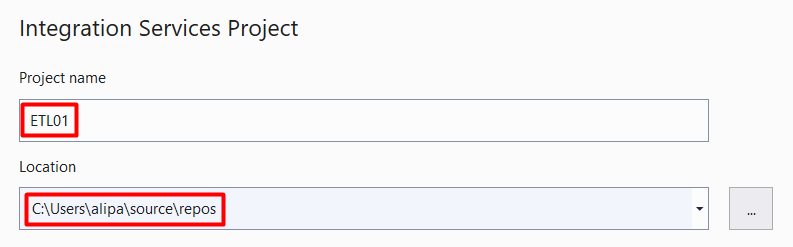
\includegraphics[width=10cm]{./img/img9.png}
\end{center}

Añadimos un paquete SSIS

\begin{center}
    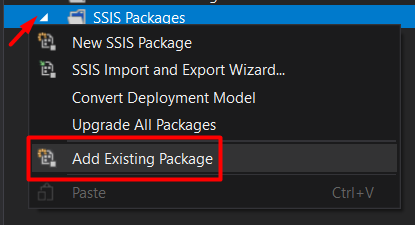
\includegraphics[width=10cm]{./img/img10.png}
\end{center}

Buscamos el paquete creado y hacemos clic en Ok

\begin{center}
    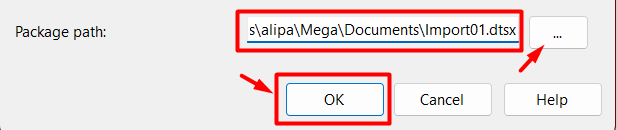
\includegraphics[width=10cm]{./img/img11.png}
\end{center}

Nos mostrará el diseño del paquete

\begin{center}
    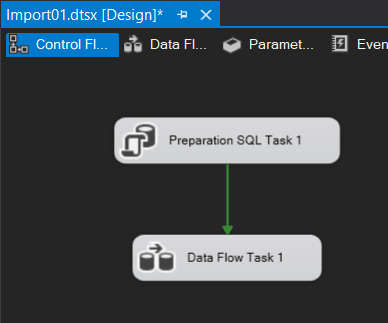
\includegraphics[width=10cm]{./img/img12.png}
\end{center}

Al hacer clic en el primer control, podemos ver las propiedades incluyendo el código SQL 

\begin{center}
    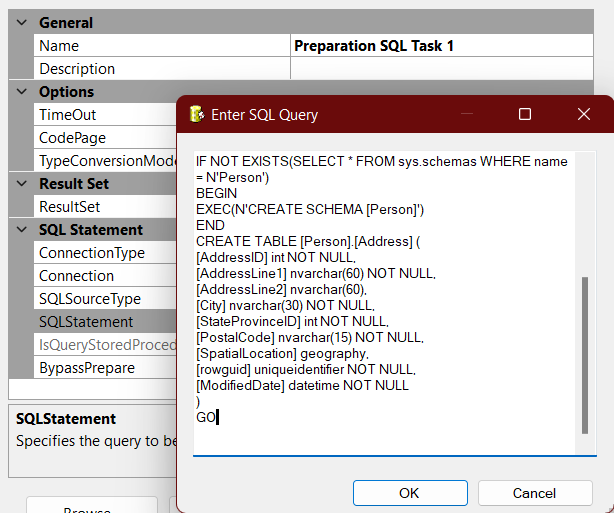
\includegraphics[width=10cm]{./img/img14.png}
\end{center}

Al hacer clic sobre el otro control, vemos el flujo de datos

\begin{center}
    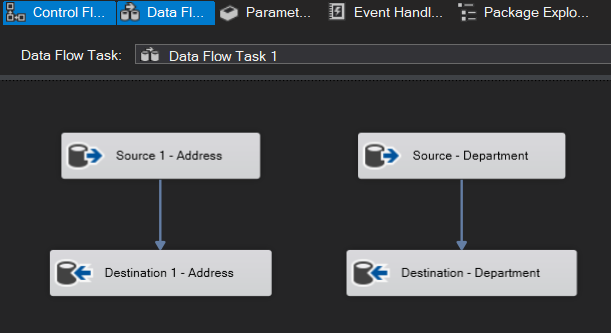
\includegraphics[width=10cm]{./img/img13.png}
\end{center}

Creamos un nuevo Integration Services Project, hacemos clic derecho en Connection Managers y luego clic en New Connection Manager

\begin{center}
    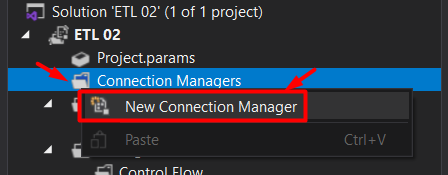
\includegraphics[width=10cm]{./img/img15.png}
\end{center}

Seleccionamos OLEDB y luego Add...

\begin{center}
    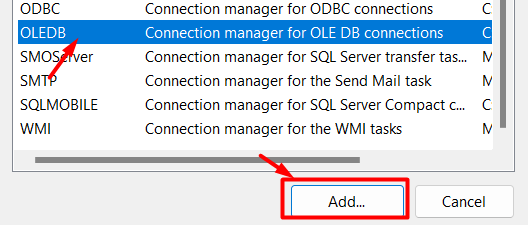
\includegraphics[width=10cm]{./img/img16.png}
\end{center}

Hacemos clic en New...

\begin{center}
    
\includegraphics[width=10cm]{./img/img17.png}
\end{center}

Buscamos la Base de datos de AdventureWorks2012 y luego clic en Ok

\begin{center}
    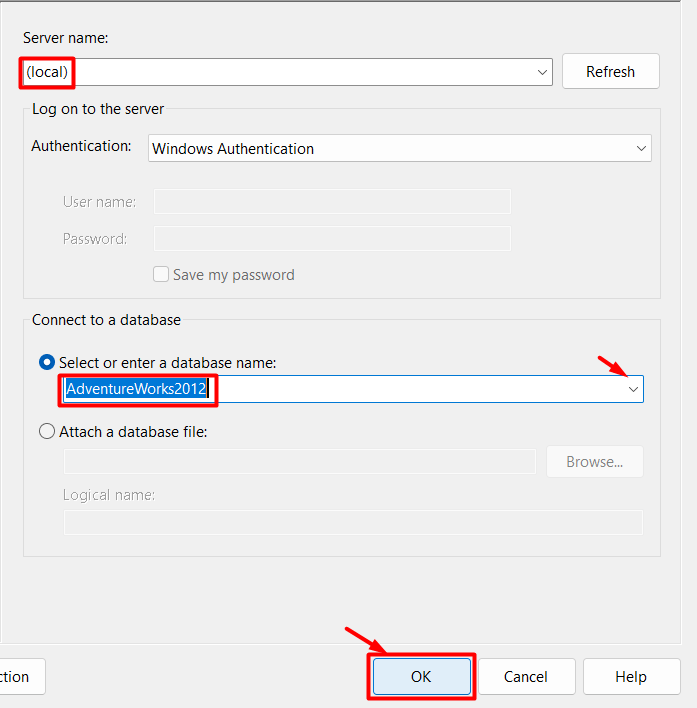
\includegraphics[width=10cm]{./img/img18.png}
\end{center}

Hacemos clic en Ok

\begin{center}
    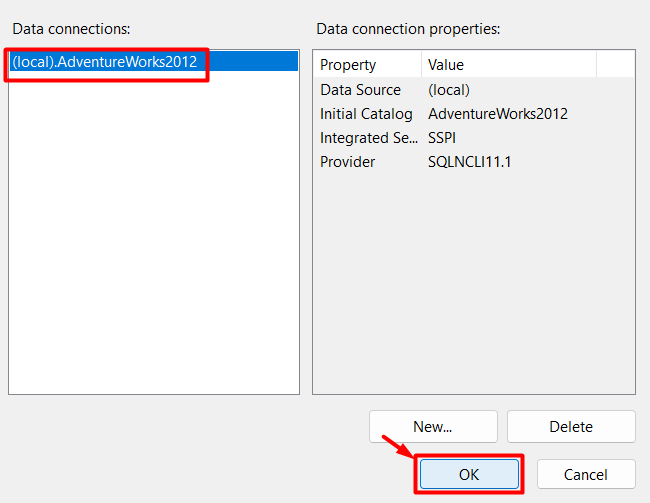
\includegraphics[width=10cm]{./img/img19.png}
\end{center}

Agregamos los controles indicados 

\begin{center}
    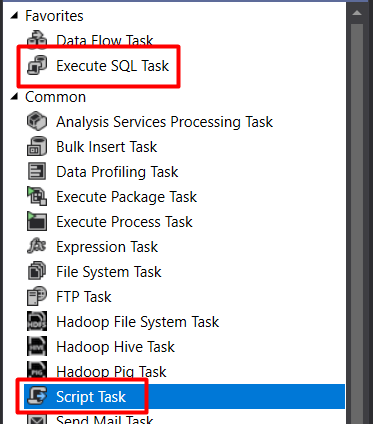
\includegraphics[width=10cm]{./img/img20.png}
\end{center}

Los enlazamos y quedarían así

\begin{center}
    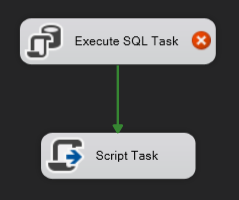
\includegraphics[width=10cm]{./img/img21.png}
\end{center}

Hacemos clic en el control, le cambiamos el nombre y la consulta SQL

\begin{center}
    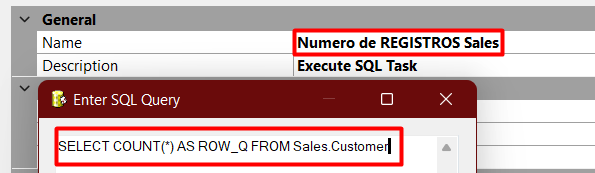
\includegraphics[width=10cm]{./img/img22.png}
\end{center}

Hacemos clic derecho en un lugar vacío y luego Variables

\begin{center}
    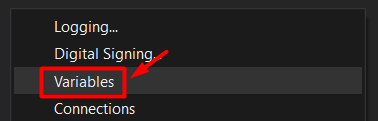
\includegraphics[width=10cm]{./img/img23.png}
\end{center}

Agregamos una nueva variable Count

\begin{center}
    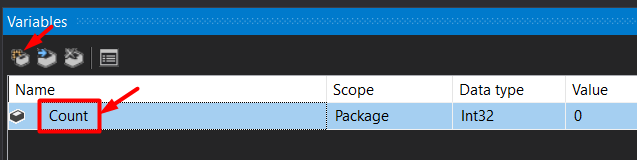
\includegraphics[width=10cm]{./img/img24.png}
\end{center}

En las opciones del Numero de REGISTROS Sales, hacemos clic en Result Set y agregamos uno

\begin{center}
    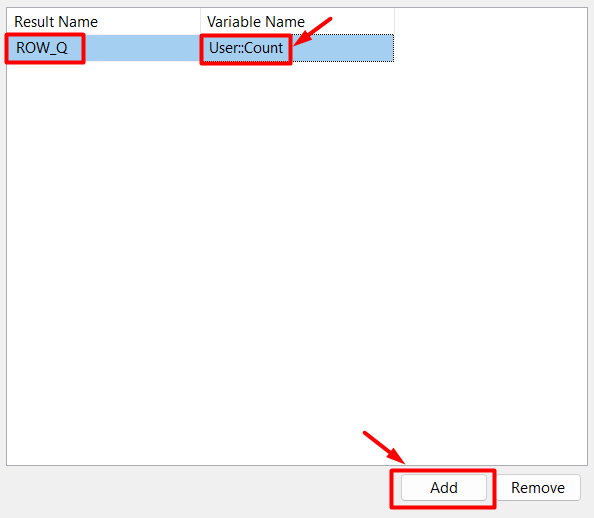
\includegraphics[width=10cm]{./img/img25.png}
\end{center}

Hacemos clic en el control Script Task y hacemos clic en los tres puntos de ReadOnlyVariables

\begin{center}
    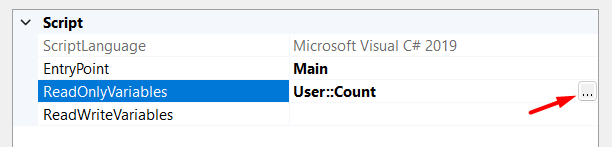
\includegraphics[width=10cm]{./img/img26.png}
\end{center}

Seleccionamos User::Count

\begin{center}
    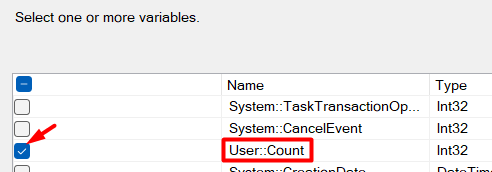
\includegraphics[width=10cm]{./img/img27.png}
\end{center}

Hacemos clic en Edit Script...

\begin{center}
    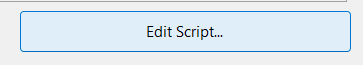
\includegraphics[width=10cm]{./img/img28.png}
\end{center}

Agregamos el código en el método Main() para que muestre el valor de la variable en un MessageBox

\begin{center}
    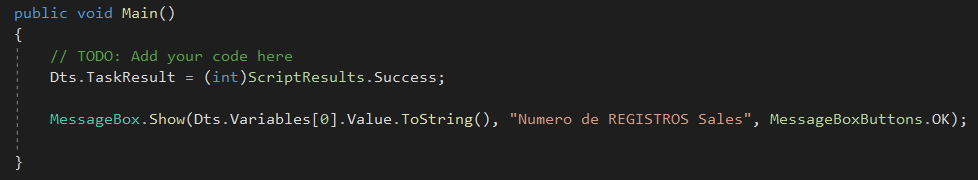
\includegraphics[width=10cm]{./img/img29.png}
\end{center}

Al ejecutar el paquete, podemos ver una ventana con el numero de registros

\begin{center}
    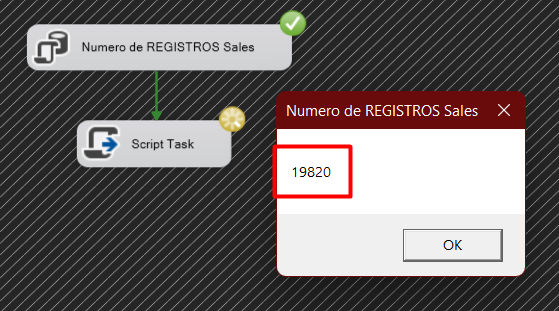
\includegraphics[width=10cm]{./img/img30.png}
\end{center}

\subsection{Cargar datos de Clientes en la Tabla Customer de BD Adventure Work.}

Crear una nueva conexión para la base de datos AdventureWorksLT2012

Crear un paquete nuevo Paquete.

\begin{center}
    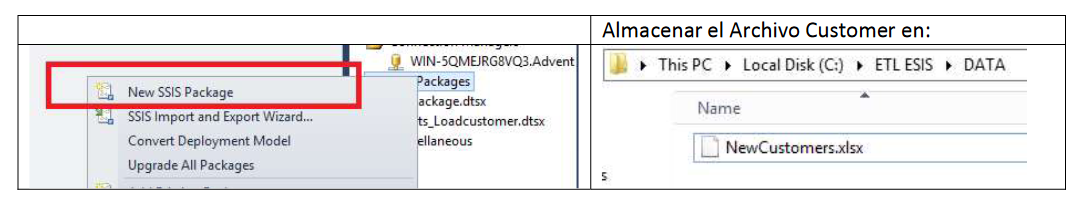
\includegraphics[width=10cm]{./img/img31.png}
\end{center}

Este es el Diagrama Final que lo haremos Juntos en CLASE.

\begin{center}
    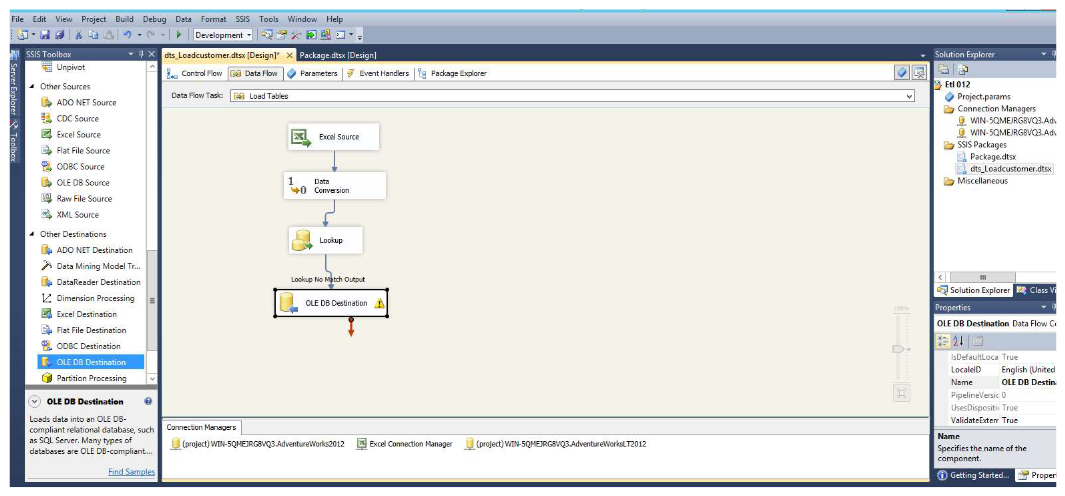
\includegraphics[width=10cm]{./img/img32.png}
\end{center}

\subsection{Ejemplo: conexión con AdventureWork (INSERTAR DATOS EN UNA TABLA)}

Agregamos los componentes indicados previamente

\begin{center}
    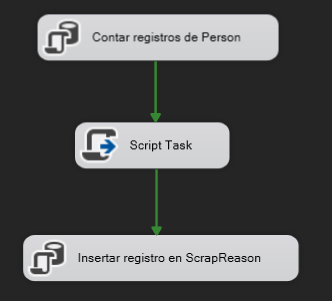
\includegraphics[width=10cm]{./img/img33.png}
\end{center}

Cambiamos el nombre, el Result Set a Single Row, elegimos la conexión y escribimos el código SQL indicado

\begin{center}
    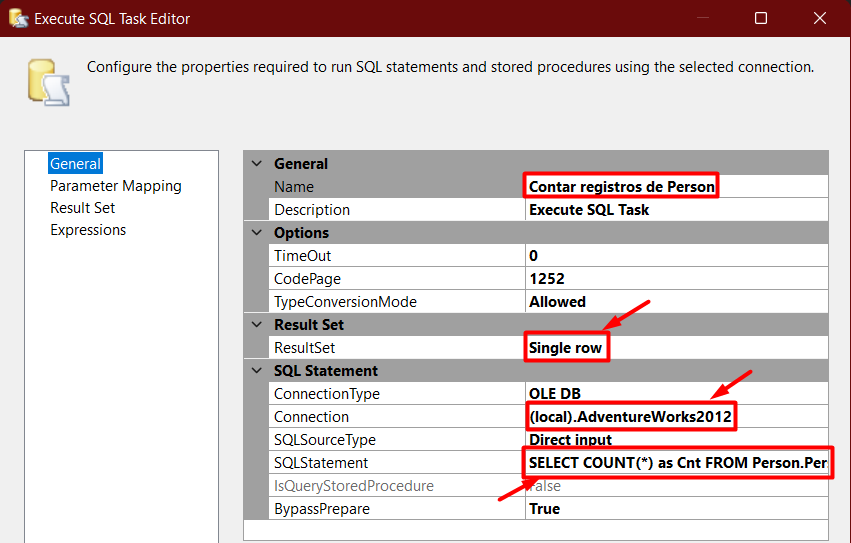
\includegraphics[width=10cm]{./img/img34.png}
\end{center}

En Result Set, agregamos la variable de lectura

\begin{center}
    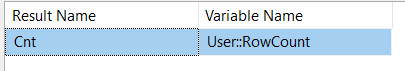
\includegraphics[width=10cm]{./img/img35.png}
\end{center}

Hacemos clic en Script Task y en ReadOnlyVariables elegimos la variable RowCount

\begin{center}
    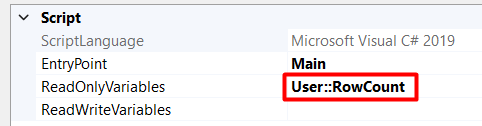
\includegraphics[width=10cm]{./img/img36.png}
\end{center}

Hacemos clic en Edit Script... y agregamos el código en el método Main()

\begin{center}
    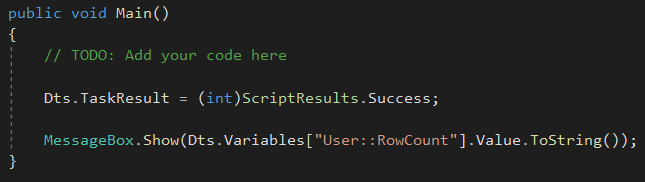
\includegraphics[width=10cm]{./img/img37.png}
\end{center}

Hacemos clic en el botón Parameters y agregamos los dos parámetros con las propiedades

\begin{center}
    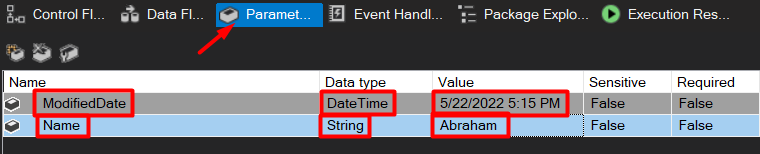
\includegraphics[width=10cm]{./img/img41.png}
\end{center}

Hacemos clic en la última tarea, cambiamos el nombre y seleccionamos la conexión

\begin{center}
    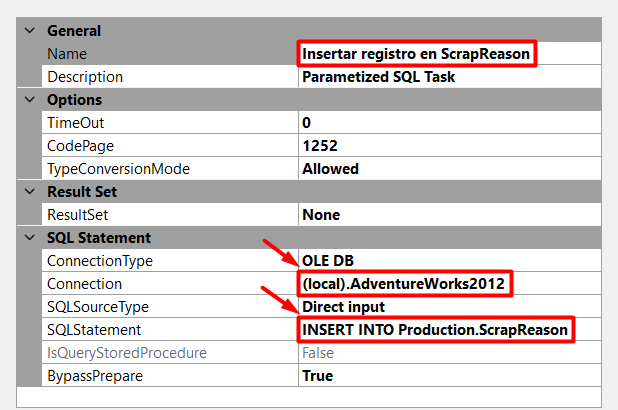
\includegraphics[width=10cm]{./img/img38.png}
\end{center}

Ingresamos el siguiente código SQL

\begin{center}
    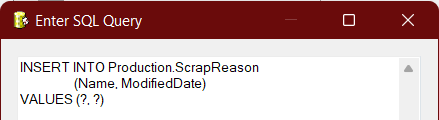
\includegraphics[width=10cm]{./img/img39.png}
\end{center}

En el apartado Parameter Mapping, agregamos dos variables con las siguientes propiedades: 

\begin{center}
    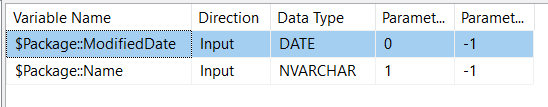
\includegraphics[width=10cm]{./img/img40.png}
\end{center}

Ejecutamos el paquete y veremos que se muestra el número de registros en Person.Person

\begin{center}
    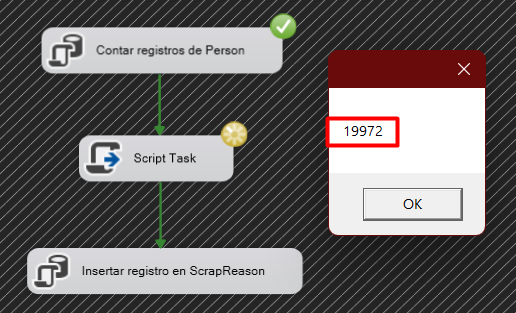
\includegraphics[width=10cm]{./img/img42.png}
\end{center}

Finalmente, todas las tareas se ejecutan correctamente

\begin{center}
    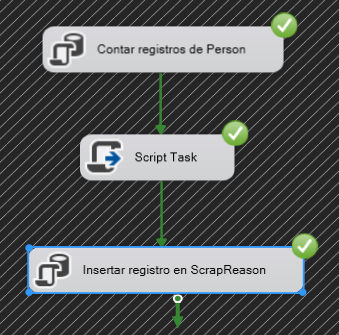
\includegraphics[width=10cm]{./img/img43.png}
\end{center}

En la base de datos, se ve el registro insertado

\begin{center}
    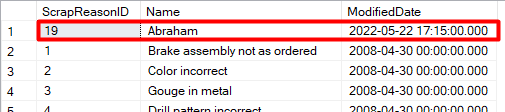
\includegraphics[width=10cm]{./img/img44.png}
\end{center}



\newpage
\section{CONCLUSIONES}
\begin{itemize}
    \item Se logró crear la base de datos para la inserción de los datos
    \item Se creó la conexión necesaria para que las tareas se apliquen a la BD
    \item Se crearon las tareas con cálculos y operaciones de la BD
\end{itemize}
\end{document}